\documentclass[11pt]{article}
\usepackage[margin=1in]{geometry}
\usepackage[T1]{fontenc}
\usepackage{lmodern}
\usepackage{amsmath,amssymb}
\usepackage{graphicx}
\usepackage{booktabs}
\usepackage{caption}
\usepackage{microtype}
\usepackage[hidelinks]{hyperref}
\captionsetup{font=small,labelfont=bf,width=0.95\textwidth}
\graphicspath{{../figs/}}
% let text share a page with a tall figure instead of forcing float-only pages
\renewcommand{\topfraction}{0.95}
\renewcommand{\bottomfraction}{0.6}
\renewcommand{\textfraction}{0.05}
\renewcommand{\floatpagefraction}{0.85}

\newcommand{\sci}[2]{$#1\times10^{#2}$}
\newcommand{\code}[1]{\texttt{#1}}
\newcommand{\rs}{r_s}
\newcommand{\vc}{v_c}

\title{Computational Physics, Homework 4:\\
Adaptive ODE integration --- the Brusselator and a supermassive black-hole
binary sinking by dynamical friction}
\author{Xuanzhe Xia \\ \texttt{xx2720@nyu.edu} \\[4pt]
\small Code: \url{https://github.com/hz-xiaxz/compphys-hw4}}
\date{November 3, 2026}

\begin{document}
\maketitle

\section*{Summary}

This assignment uses two adaptive ODE integrators. In the first part
(Newman, Exercise~8.18) I solved the Brusselator model of an oscillating
chemical reaction for $a=1$, $b=3$. I used the Bulirsch--Stoer method with
recursive interval halving to an accuracy of $10^{-10}$ per unit time. The
concentrations settle onto a limit cycle with period $\approx7.1$: $y$ builds
up slowly and then collapses within about one time unit while $x$ spikes. The
139 accepted intervals range from 0.625 to 0.0195 in width and crowd together
at these fast switches. A tighter run confirms that the error at $t=20$ is
below \sci{7}{-10}.

In the second part I followed one black hole of an equal-mass
supermassive binary ($M=1.05\times10^8M_\odot$ each, fixed by
$\rs=10^{-5}$\,pc) sinking under dynamical friction. I used adaptive RK4 and
stopped when the separation reached the Schwarzschild radius. A
frictionless test orbit with pericentre $\rs$ (eccentricity
$1-2\times10^{-7}$) sets the tolerance at $\delta=10^{-10}$: over 10 orbits
the energy is conserved to \sci{6}{-7} and the pericentre to \sci{4}{-11},
with 6800 steps per orbit. For $A=B=1$ the binary reaches $\rs$ after
15.7\,Myr and 30 pericentre passages. It gets there by becoming extremely
eccentric ($1-e\sim10^{-6}$) while its semi-major axis is still 4.6\,pc,
because the friction removes angular momentum during the slow apocentre
phases. The time to reach $\rs$ is mainly a function of $B/A$ and has a
minimum of 6.2\,Myr at $B/A\approx0.44$, where the drag is critically damped.
For strong friction (small $B/A$) the hole sinks radially at terminal velocity
in a time $\frac43A/B$. For weak friction (large $B/A$) it needs many orbits
and the time grows as $12.3\,B/A$, reaching 374\,Myr at $B/A=20$. The time
depends on the initial speed only in the orbiting regime, where it rises with
$v_0$ up to $v_0\approx v_c$. Changing $A$ at fixed $B/A$ alters the time by
up to 25\% near $B/A\sim1$, where the hole's speed crosses $B^{1/3}$ and the
drag changes from linear to $\propto v^{-2}$. Elsewhere the effect is a few
percent or less.

\section*{Methods}

\subsection*{Problem 1: the Brusselator (Exercise 8.18)}

The Brusselator is a model chemical oscillator:
\begin{equation}
\frac{dx}{dt} = 1-(b+1)x+ax^2y, \qquad \frac{dy}{dt} = bx-ax^2y .
\end{equation}
Its only fixed point is $(x,y)=(1,b/a)$. The Jacobian there,
$\bigl(\begin{smallmatrix} b-1 & a\\ -b & -a\end{smallmatrix}\bigr)$, has trace
$b-1-a$ and determinant $a$. For $a=1$, $b=3$ the eigenvalues are
$\tfrac12\pm\tfrac{\sqrt3}{2}i$, so the fixed point is an unstable spiral and
solutions are attracted to a limit cycle.

I solved the equations from $t=0$ to $20$ with $x=y=0$ at $t=0$, using the
Bulirsch--Stoer method with recursive interval halving that the exercise asks
for. An interval of width $H$ is integrated with the modified midpoint method
using $n=1,2,\dots,8$ substeps, giving the estimates $R_{n,1}$. These are
Richardson-extrapolated with
\begin{equation}
R_{n,m+1} = R_{n,m} + \frac{R_{n,m}-R_{n-1,m}}{[n/(n-1)]^{2m}-1},
\end{equation}
and the last correction term, applied to get $R_{n,n}$, is taken as the error
estimate $\epsilon$. The interval is accepted with the value $R_{n,n}$ as soon
as $\max(|\epsilon_x|,|\epsilon_y|) < H\delta$ with
$\delta=10^{-10}$ per unit time. If this does not happen by $n=8$, the function
calls itself on the two halves of the interval, starting from $H=20$.
Recursion places short intervals only where they are needed. On the first
tries ($H=20$, $10$, \dots) the midpoint method overflows. The resulting
\code{nan} fails the error test, so those intervals are simply split as well.

I checked the result against a run with $\delta=10^{-12}$. The same method on a
fine fixed grid of 4000 intervals gives the smooth curves drawn in the figure.

\subsection*{Problem 2: a black-hole binary sinking by dynamical friction}

\paragraph{Equations and units.} Two black holes of equal mass $M$ sit at
$\pm\mathbf r$, separated by $2r$, so one of them feels $GM/(2r)^2$. With
dynamical friction (DF) from the surrounding stars,
\begin{equation}
\ddot{\mathbf r} = -\frac{GM}{4r^3}\,\mathbf r
  - \frac{A}{v^3+B}\,\mathbf v . \label{eq:eom}
\end{equation}
The homework sheet writes both terms with a plus sign. I take gravity as
attractive and the DF term as a drag opposite to $\mathbf v$, which is the
physical meaning. Equation~\eqref{eq:eom} is a Kepler problem with effective
$GM'=1/4$, so the circular speed at $r=1$ is $v_c=1/2$. The DF term is the
interpolation formula of the sheet. For $v^3\ll B$ it is a linear drag
$-(A/B)\mathbf v$, the slow-body limit of Chandrasekhar's formula with
$B\sim\sigma^3$. For $v^3\gg B$ it falls off as $A/v^2$.

I used $G=M=1$ with a length unit of 100\,pc. The Schwarzschild radius
$\rs = 2GM/c^2 = 10^{-7}$ then fixes the mass of each hole,
$M = \rs c^2/2G = 1.05\times10^8\,M_\odot$. The velocity unit is
$\sqrt{GM/100\,\mathrm{pc}} = 67.0$\,km\,s$^{-1}$ and the time unit is
$1.459$\,Myr, which I used to convert times to Myr.

\paragraph{Integrator.} I used fourth-order Runge--Kutta with the adaptive step
of Newman Sec.~8.4. Each step of size $2h$ is done twice, as two steps of $h$
and as one step of $2h$. The position error estimate is
$\epsilon = |\mathbf r_1-\mathbf r_2|/30$. If $\rho = h\delta/\epsilon \ge 1$
the step is accepted, using the two-step result, and the next $h$ is
$h\rho^{1/4}$, at most $2h$. Otherwise the step is redone with $h\rho^{1/4}$.
The integrator is compiled with \code{numba}, so a run of $10^7$ steps takes
seconds. A run stops when an accepted step has $r\le\rs$. Pericentres are also
detected where $\mathbf r\cdot\mathbf v$ changes sign from negative to positive.
At each one, the pericentre of the osculating Kepler orbit,
\begin{equation}
r_p = \frac{L^2}{GM'(1+e)},\qquad e=\sqrt{1+2EL^2/GM'^2},
\end{equation}
is compared with $\rs$ too, so a pericentre that falls between two steps is not
missed. This form avoids the cancellation in $a(1-e)$ when $e\to1$. Near
pericentre the DF is negligible: at $r=\rs$ it is $10^{-20}$ of gravity, so the
osculating $r_p$ is exact there. The black hole starts at $(1,0)$ with velocity
$v_0\hat{\mathbf y}$, where $v_0 = 0.8v_c=0.4$ in all runs with friction.

\paragraph{(a) Choosing $\delta$.} Without friction, an orbit with apocentre 1
and pericentre $\rs$ needs
$v_0 = \sqrt{2GM'\rs/(1+\rs)} = 2.236\times10^{-4}$. It has eccentricity
$1-2\times10^{-7}$ and period $T=4.443$. At pericentre the speed is 2236 and
the passage lasts $\rs/v_p \approx 5\times10^{-11}$, a dynamic range of
$10^{11}$ in time scale. I followed 10 orbits for
$\delta=10^{-6},\dots,10^{-11}$. At every apocentre I measured the energy $E$
and angular momentum $L$, and at every pericentre the pericentre distance.

\paragraph{(c, d) Parameter scans.} For (c) I ran a $12\times12$ grid with $A$
and $B$ logarithmically spaced in $[0.5,10]$, so $B/A$ spans $0.05$--$20$.
For (d) I varied $v_0/v_c$ from $0.1$ to $1.3$ for six $(A,B)$ pairs: two
pairs with different $A$ at each of $B/A = 0.2$, $1$ and $5$. I also scaled $A$ and $B$ together at
fixed $B/A$. The runs are independent and are spread over CPU cores with
\code{multiprocessing}.

\section*{Results}

\subsection*{Problem 1: the Brusselator}

\begin{figure}[t]
\centering
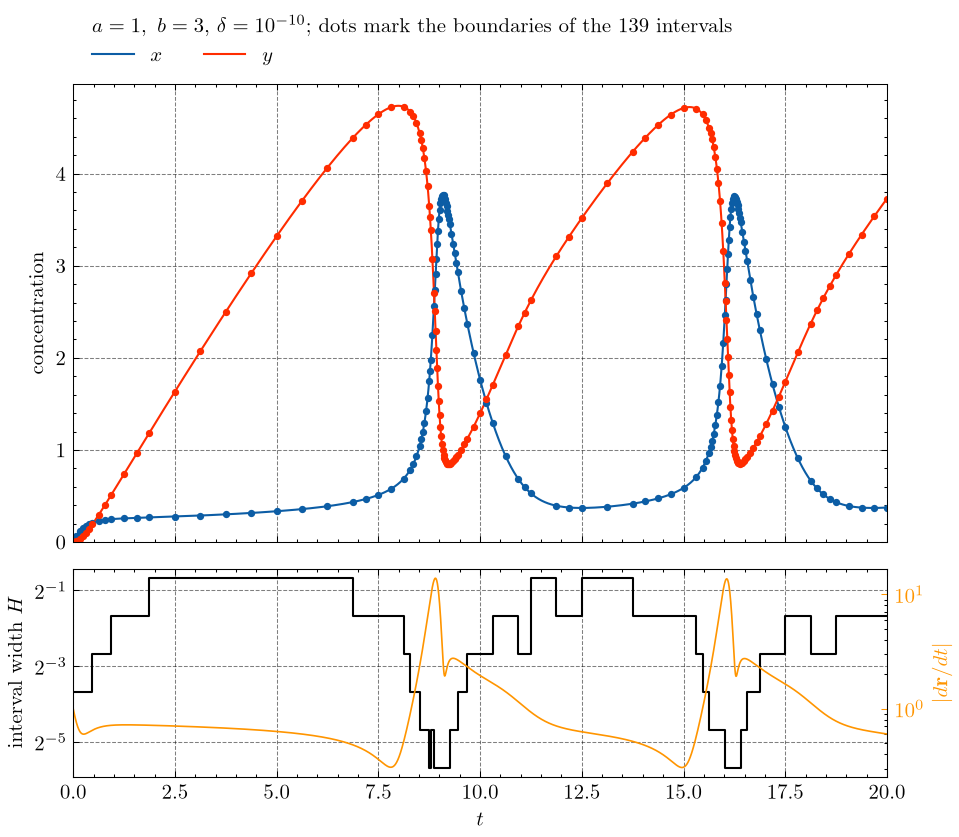
\includegraphics[width=0.8\textwidth]{problem1_brusselator.png}
\caption{Top: Brusselator concentrations $x$ (blue) and $y$ (red) for $a=1$,
$b=3$, $x(0)=y(0)=0$. Dots mark the ends of the 139 intervals accepted by the
recursive Bulirsch--Stoer solver at $\delta=10^{-10}$ per unit time. Bottom:
width $H$ of each interval (black, log$_2$ scale) and the speed
$|d\mathbf r/dt| = \sqrt{\dot x^2+\dot y^2}$ along the solution (green, right axis).}
\label{fig:bruss}
\end{figure}

Figure~\ref{fig:bruss} shows the solution. Starting from zero, $x$ quickly
levels off near $0.25$, while $y$ grows almost linearly to $4.7$ by $t\approx8$.
Then $x$ shoots up to a spike of $3.8$ and $y$ collapses to $0.85$ within about
one time unit. The same cycle then repeats with period $\approx 7.1$: a slow
build-up of $y$ followed by a sharp switch. This is the limit cycle that the
unstable fixed point $(1,3)$ implies.

The solver accepted 139 intervals, with widths from $20/2^{5}=0.625$ down to
$20/2^{10}=0.0195$. The accepted intervals used $n=5$--$8$ midpoint substeps,
7.7 on average. As the exercise predicts, the dots crowd together at the
switches near $t\approx 9$ and $16$, where the variables change fastest. In the
bottom panel the interval width tracks the speed: the correlation between
$\log H$ and $\log|d\mathbf r/dt|$ is $-0.80$. Intervals average 0.035 where the
speed is above its median and 0.25 elsewhere. At $t=20$ the result is
$x=0.3751036102$, $y=3.7279158358$. Its difference from the $\delta=10^{-12}$
run is \sci{5}{-11} in $x$ and \sci{7}{-10} in $y$, inside the
$\delta\times20=2\times10^{-9}$ target, so the per-interval error estimates are
reliable.

\subsection*{Problem 2(a): choosing the tolerance}

\begin{figure}[t]
\centering
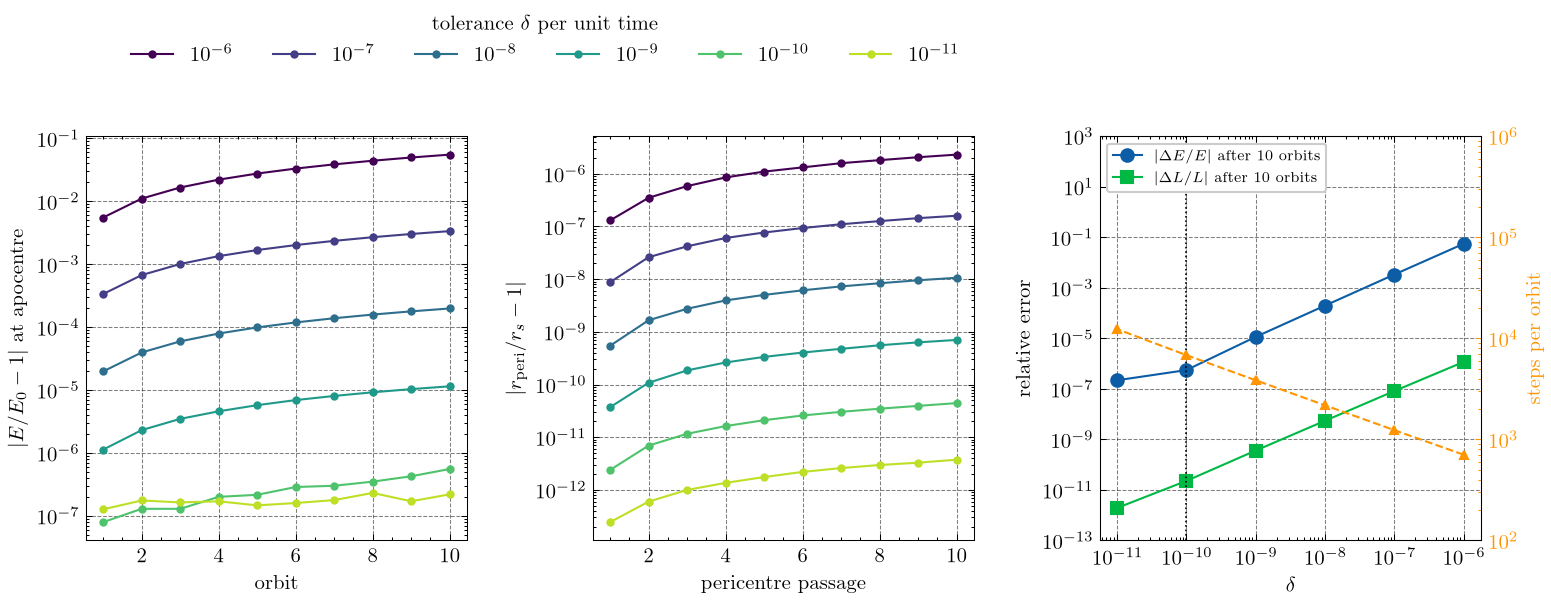
\includegraphics[width=\textwidth]{problem2a_tolerance.png}
\caption{Kepler orbit without friction, with apocentre 1 and pericentre
$\rs=10^{-7}$ (eccentricity $1-2\times10^{-7}$), followed for 10 orbits. Left:
relative energy error at each apocentre. Middle: relative error in the
pericentre distance at each passage. Right: error after 10 orbits (left axis)
and RK4 steps per orbit (right axis) against $\delta$. The dotted line marks
the adopted $\delta=10^{-10}$.}
\label{fig:tol}
\end{figure}

\begin{table}[b]
\centering\small
\begin{tabular}{lrrrrr}
\toprule
$\delta$ & steps/orbit & $\Delta E/E$ & $\Delta L/L$ & max $|r_p/\rs-1|$ & period error\\
\midrule
$10^{-6}$  &   706 & \sci{-5.5}{-2} & \sci{-1.2}{-6}  & \sci{2}{-6}   & \sci{2}{-1}\\
$10^{-7}$  &  1236 & \sci{-3.4}{-3} & \sci{-8}{-8}    & \sci{2}{-7}   & \sci{1}{-2}\\
$10^{-8}$  &  2177 & \sci{-2.0}{-4} & \sci{-5}{-9}    & \sci{1}{-8}   & \sci{7}{-4}\\
$10^{-9}$  &  3851 & \sci{-1.1}{-5} & \sci{-4}{-10}   & \sci{7}{-10}  & \sci{4}{-5}\\
$10^{-10}$ &  6830 & \sci{-5.5}{-7} & \sci{-2}{-11}   & \sci{4}{-11}  & \sci{2}{-6}\\
$10^{-11}$ & 12343 & \sci{+2.2}{-7} & \sci{-2}{-12}   & \sci{4}{-12}  & \sci{-1}{-6}\\
\bottomrule
\end{tabular}
\caption{Conservation over 10 orbits of the $r_p=\rs$ Kepler orbit
($T=4.443$). $\Delta E$ and $\Delta L$ are measured at the 10th apocentre; the
period error is the mean spacing of pericentre passages minus $T$.}
\label{tab:tol}
\end{table}

Figure~\ref{fig:tol} and Table~\ref{tab:tol} show the test orbit. The step
size spans eleven decades, from $\sim\!0.1$ at apocentre to $\sim\!10^{-12}$ at
pericentre, yet the cost is only a few thousand steps per orbit. The cost grows
as $\delta^{-1/4}$, as expected for a fourth-order method. The adaptive scheme
keeps the angular momentum, and hence the pericentre distance, extremely well:
even at $\delta=10^{-6}$ the pericentre stays at $\rs$ to \sci{2}{-6}. Energy is
the weak point. Each pericentre passage leaves a small energy error that
accumulates linearly with the number of orbits (left panel). The error scales
as roughly $\delta^{1.25}$, from 5\% after 10 orbits at $\delta=10^{-6}$ to
\sci{5.5}{-7} at $\delta=10^{-10}$. Below $\delta\approx10^{-11}$ round-off
takes over: the energy error stops falling. At $\delta=10^{-12}$ the step at
pericentre becomes smaller than the spacing of doubles near $t=2.2$, so $t+h=t$
and the integration stalls. The code detects this and stops.

I adopted $\delta=10^{-10}$. Over 10 orbits the energy changes by
\sci{6}{-7}, the pericentre distance by \sci{4}{-11}, the apocentre by
\sci{6}{-7} and the period by \sci{2}{-6}, so there is no appreciable loss of
accuracy. In the friction runs, the time to reach $\rs$ changes by only
\sci{2.5}{-7} between $\delta=10^{-9}$ and $10^{-11}$ for $A=B=1$, and by
\sci{1.2}{-5} between $10^{-9}$ and $10^{-10}$ for the slowest case
($A=0.5$, $B=10$, 14\,000 pericentre passages).

\subsection*{Problem 2(b): the orbit for $A=B=1$}

\begin{figure}[t]
\centering
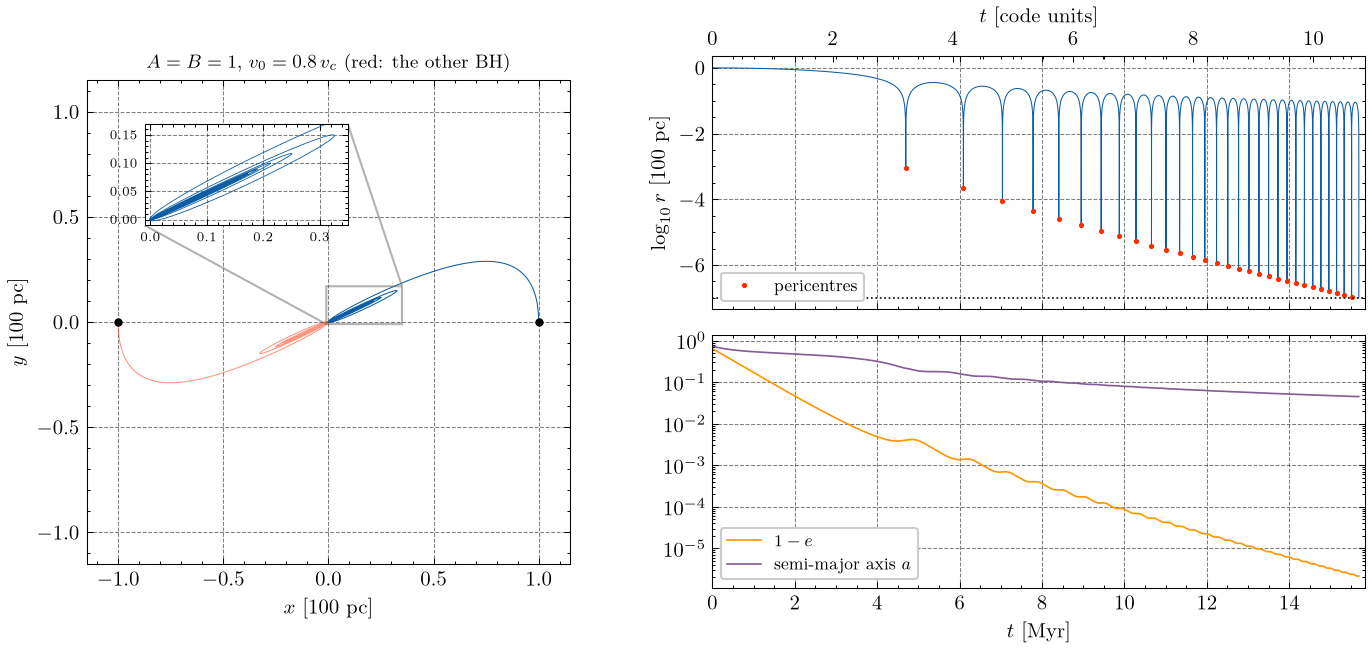
\includegraphics[width=\textwidth]{problem2b_orbit.png}
\caption{Orbit for $A=B=1$, $v_0=0.8v_c$. Left: path of the black hole (blue)
and its partner (red), with a zoom on the inner orbits. Top right:
$\log_{10}r$ against time, with the pericentres marked and $\rs$ dotted.
Bottom right: $1-e$ and semi-major axis $a$ of the osculating Kepler orbit.}
\label{fig:orbit}
\end{figure}

With $A=B=1$ the black hole reaches $\rs$ at $t=10.756$, or
\textbf{15.7\,Myr}, after 30 pericentre passages and \sci{1.4}{5} RK4 steps
(Fig.~\ref{fig:orbit}). The first infall does most of the work. Starting at
$v=0.4$, where the drag is almost linear with rate $A/(v^3+B)\approx0.94$, the
hole loses 95\% of its angular momentum ($L$ falls from 0.40 to 0.021) before
the first pericentre at $r_p=8.7\times10^{-4}$. From then on the orbit is
nearly radial. At each pericentre the speed is so high that the drag
($\propto A/v^2$) is negligible. Near apocentre the hole is slow, and the drag
removes angular momentum and energy. Since the drag is parallel to
$\mathbf v$, its torque gives exactly
$\dot L = -AL/(v^3+B)$, so $L$, and with it $r_p\simeq L^2/2GM'$, decays
almost exponentially. As a result $\log r_p$ falls roughly linearly with time,
and $1-e$ falls from 0.64 to \sci{2}{-6}. The semi-major axis shrinks only
from 0.74 to 0.046 (4.6\,pc). The binary does not reach $\rs$ by shrinking its orbit as a whole. It
gets there by becoming extremely eccentric, so that its pericentre plunges to
$\rs$ while its apocentre stays at parsec scales. The inset shows that the
orientation of the orbit also rotates slowly.

\subsection*{Problem 2(c): dependence on $B/A$}

\begin{figure}[t]
\centering
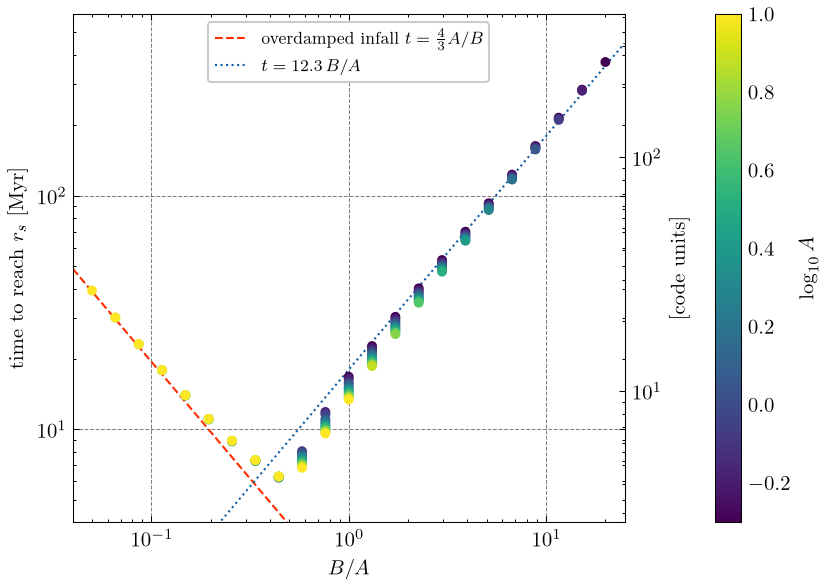
\includegraphics[width=0.72\textwidth]{problem2c_ratio.png}
\caption{Time for the binary to reach $\rs$ against $B/A$, for 144 runs with
$A,B$ on a logarithmic $12\times12$ grid in $[0.5,10]$ and $v_0=0.8v_c$.
Colour shows $\log_{10}A$. Red dashed: the overdamped terminal-velocity infall
time $\tfrac43A/B$. Blue dotted: $12.3\,B/A$, the geometric mean of $t/(B/A)$
over the runs with $B/A>4$.}
\label{fig:ratio}
\end{figure}

Figure~\ref{fig:ratio} shows a V shape in log--log axes. The time to reach $\rs$
is shortest, \textbf{6.2\,Myr} ($t=4.26$), at $B/A\approx0.44$. It grows on
both sides, up to 39\,Myr at $B/A=0.05$ and 374\,Myr at $B/A=20$. The reason is
the same as for a damped oscillator. At low speed the DF is a linear drag with
rate $\gamma=A/B$, and the motion is set by how $\gamma$ compares with the
orbital frequency $\Omega=\sqrt{GM'/r^3}=0.5$ at $r=1$.

\emph{Strong friction, $B/A\lesssim0.4$ (overdamped).} The drag kills the
initial velocity within a time $B/A$, so the hole never completes an orbit (no
pericentre passages in these runs). It sinks radially at the terminal velocity
where drag balances gravity, $v=GM'/(\gamma r^2)$. Integrating
$\dot r=-GM'B/(Ar^2)$ from $r=1$ gives
\begin{equation}
t_{\rm sink}=\frac{A}{3GM'B}=\frac43\,\frac{A}{B},
\end{equation}
which matches the runs with $B/A<0.1$ to within 2.5\%. Here \emph{more}
friction means a \emph{longer} time, because the hole falls more slowly through
a more viscous medium.

\emph{Weak friction, $B/A\gtrsim1$ (underdamped).} The hole keeps orbiting,
and as in (b) it must lose angular momentum from $L_0=0.4$ down to
$L_s=\sqrt{2GM'\rs}=2.2\times10^{-4}$. That is $\ln(L_0/L_s)\approx7.5$
$e$-folds. Because $\dot L=-AL/(v^3+B)$ exactly,
\begin{equation}
\ln\frac{L_0}{L_s} = \frac{A}{B}\int_0^{t}\frac{dt'}{1+v^3/B},
\end{equation}
so $t\ge7.5\,B/A$, with equality for a purely linear drag. The measured times
follow $t\approx12.3\,B/A$ (11.6--12.8 for $B/A>4$). Hence the time average of
$1/(1+v^3/B)$ is about $7.5/12.3=0.6$. As the orbit shrinks, the typical speed
$\sqrt{GM'/a}$ rises towards $B^{1/3}$, and the drag is almost switched off
during the fast pericentre passages. The number of orbits grows quickly, from 23--87
pericentre passages at $B/A=1$ to 14\,000 at $B/A=20$, as the orbit becomes
very eccentric and its period shrinks.

The fastest sinking, near $B/A\approx0.44$, is the critically damped case. The
drag rate $\gamma\approx2.3$ is a few times $\Omega$, so the hole loses its
angular momentum in a single infall, and the radial sinking is not yet slowed
by viscosity. At $B/A=0.58$ the runs make 3 pericentre passages, and above that
the orbiting regime begins.

\subsection*{Problem 2(d): initial velocity, and $A$ and $B$ separately}

\begin{figure}[t]
\centering
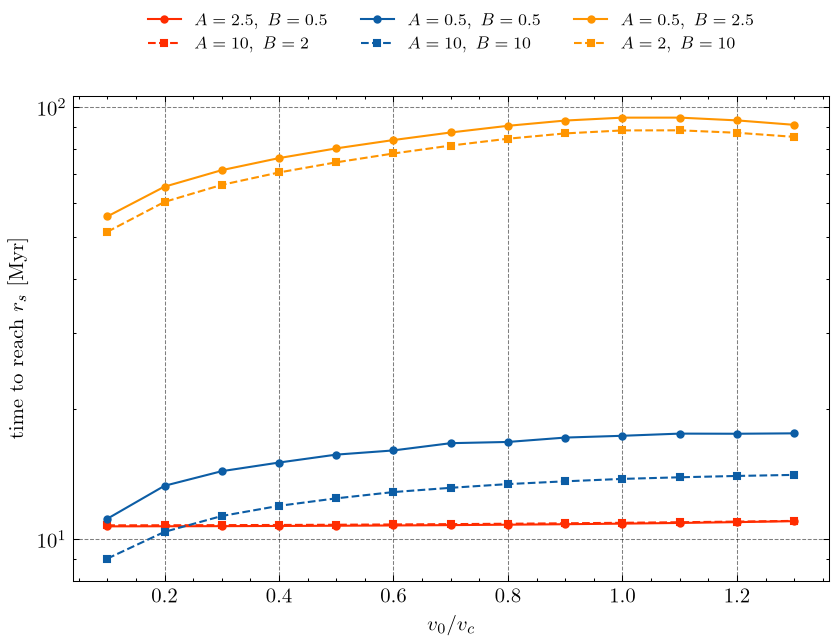
\includegraphics[width=0.72\textwidth]{problem2d_v0.png}
\caption{Time to reach $\rs$ against the initial speed $v_0/v_c$, for pairs of
$(A,B)$ with the same ratio (same colour): $B/A=0.2$ (red), $1$ (blue) and $5$
(orange). Solid lines have the smaller $A$, dashed lines the larger.}
\label{fig:v0}
\end{figure}

\paragraph{Initial velocity.} Figure~\ref{fig:v0} shows that the answer depends
on $v_0$ only when the friction is weak. In the overdamped case ($B/A=0.2$) the
initial velocity is erased within $t\sim B/A$, and $t$ changes by only 3\%
between $v_0=0.1v_c$ and $1.3v_c$. For $B/A=1$ and $5$, $t$ rises with $v_0$:
from 7.6 to 11.9 ($A=B=0.5$) and from 38 to 65 ($A=0.5$, $B=2.5$) as $v_0$ goes
from $0.1v_c$ to $v_c$. The reason is that a slower start means less initial
angular momentum, so fewer $e$-folds of $L$ are needed. For $B/A=5$ the time
peaks at $v_0\approx v_c$, the nearly circular start, and falls slightly beyond
it. So the qualitative picture of (c) is unchanged, but the
weak-friction times quoted there hold for $v_0=0.8v_c$. For a nearly radial
start ($v_0=0.1v_c$) they are 33--38\% shorter.

\paragraph{$A$ and $B$ separately.} The results depend \emph{mainly}, but not
only, on $B/A$. In Fig.~\ref{fig:ratio} the runs with equal $B/A$ but different
$A$ are colour-coded. Their spread is below 1\% for $B/A<0.45$, peaks at 25\%
near $B/A=1$, and falls to 2\% at $B/A=11.6$. Scaling $A$ and $B$ together
from 0.5 to 10 at $B/A=1$ lowers $t$ from 11.5 to 9.2. At $B/A=5$ it lowers $t$
from 62.1 to 58.6, and at $B/A=0.2$ it leaves $t$ unchanged at 7.42--7.44. The
formula explains this. For $v^3\ll B$ the drag $-(A/B)\mathbf v$ depends only
on the ratio. For $v^3\gg B$ it becomes $-A\mathbf v/v^3$, which depends on $A$
alone, and the crossover speed is $B^{1/3}$ (0.8 for $B=0.5$, 2.2 for $B=10$).
At fixed $B/A$, larger values of both keep the drag linear, and therefore
strong, up to higher speeds, so the hole sinks somewhat faster. The ratio
dominates whenever the hole spends most of its time at $v\ll B^{1/3}$. That is
the case in the overdamped infall, which is slow everywhere, and in the
weak-friction limit, where the drag acts during the long, slow apocentre
phases. Near $B/A\sim1$ the hole moves at speeds comparable to $B^{1/3}$ while
the drag is acting, so the individual values matter most there.

\section*{Code}

All code, the figures and the numerical outputs are in a GitHub repository:
\begin{center}
\url{https://github.com/hz-xiaxz/compphys-hw4}
\end{center}
The scripts are plain Python (NumPy, Numba, Matplotlib, SciencePlots) managed
with \code{uv}:
\begin{itemize}
\item \code{problem1.py}: recursive Bulirsch--Stoer solution of the
Brusselator, the accuracy check, and \path{figs/problem1_brusselator.png}.
\item \code{bhorbit.py}: the adaptive RK4 integrator for
Eq.~\eqref{eq:eom} (compiled with Numba), pericentre detection, and the unit
conversion.
\item \code{problem2.py}: parts (a)--(d) of Problem 2 and
\path{figs/problem2a_tolerance.png}, \path{problem2b_orbit.png},
\path{problem2c_ratio.png} and \path{problem2d_v0.png}.
\item \code{plotstyle.py}: shared figure style. \code{results/} holds the
printed output of each script, and \code{writeup/} holds the source of this
document.
\end{itemize}
Running \code{uv sync} followed by \code{uv run python problemN.py} reproduces
every figure and number quoted here. \code{problem2.py} takes about 4 minutes on
8 cores.

\end{document}
